\chapter{Electron and muon consistency in the control regions}
\label{app:ch8_emu}

The electron and muon channels in $\CRW$ are combined as described in Section~\ref{sec:ch8_wjets}.
The difference between their data/MC ratios is investigated here.
Before fitting, the ratios in $\CRW$-$\NonRes$ are $1.00\pm0.09$ and $0.80\pm0.08$ for the electron and muon channels, respectively, corresponding to a $1.7\sigma$ difference.
The uncertainties in this study are statistical only.

The scale factors in the two channels are first checked and found to be applied correctly.
The data/MC ratio is then examined after each cut.
The difference appears after the $50<\pT^{j_1}<250~\GeV$ requirement in $\CRW$-$\NonRes$.
The leading-jet $\pT$ distributions are compared between channels, separately for data and simulation, in Figure~\ref{fig:app_ch8_emu_ratio}.
The electron yield is slightly higher in data and slightly lower in simulation.
An upward fluctuation is observed in the electron data around $80$--$100~\GeV$.

The simulated event weights, including cross-section normalisation, efficiency scale factors and pile-up weights, are examined as a function of leading-jet $\pT$ in Figure~\ref{fig:app_ch8_emu_weights}.
A small number of events have weights of approximately 30.
Most lie below $50~\GeV$, but one such event is found above this threshold in the selected muon sample, with no corresponding event in the electron sample.
It increases the weighted muon prediction and lowers its data/MC ratio.

\begin{figure}[htpb]
    \centering
    \begin{subfigure}{0.49\linewidth}
        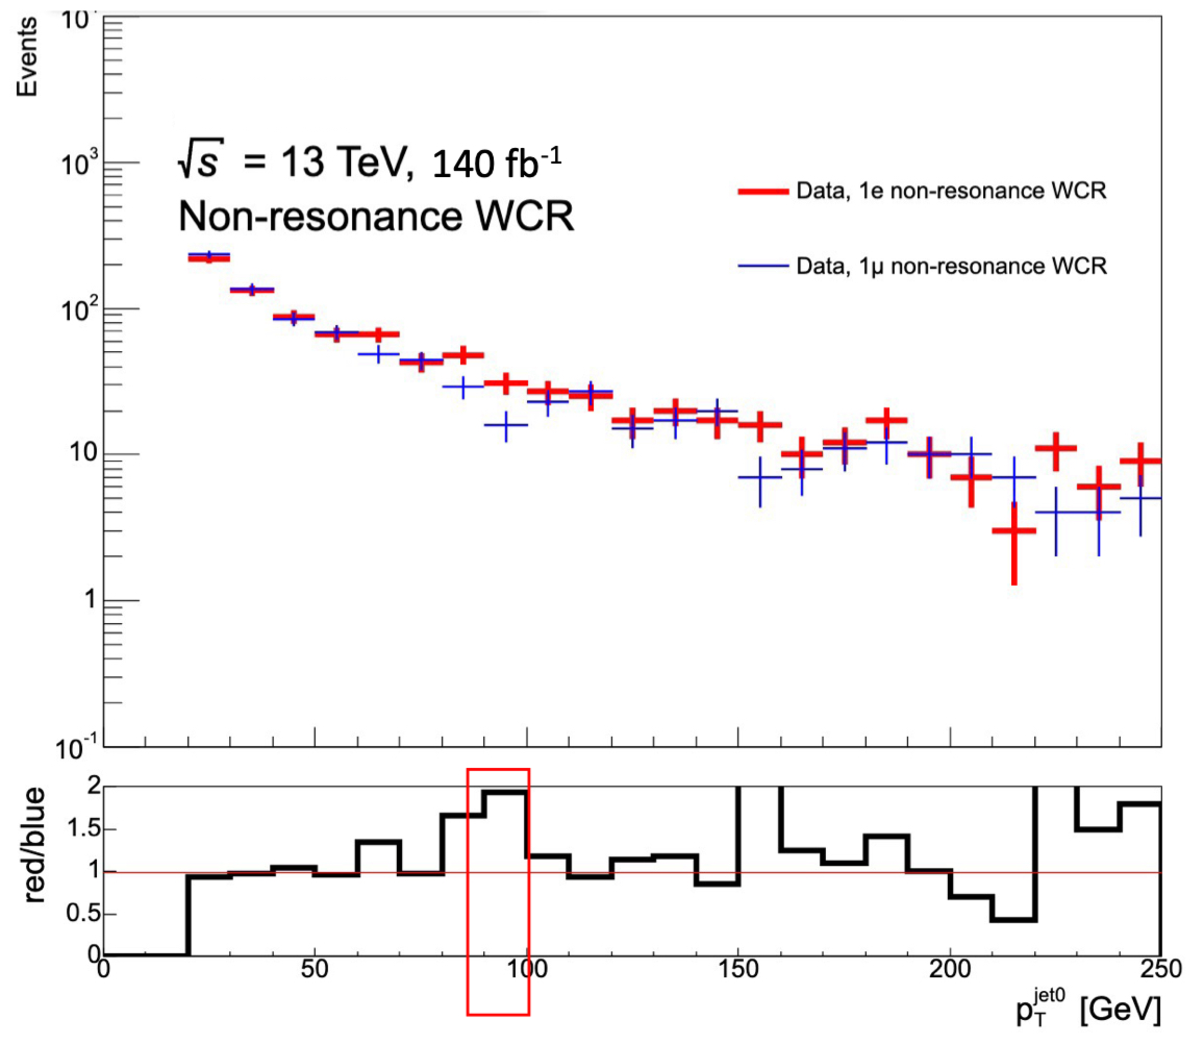
\includegraphics[width=\linewidth]{Figs/CH8/studies/WCR_emuRatio_Data.pdf}
        \caption[]{Data.}
    \end{subfigure}\hfill
    \begin{subfigure}{0.49\linewidth}
        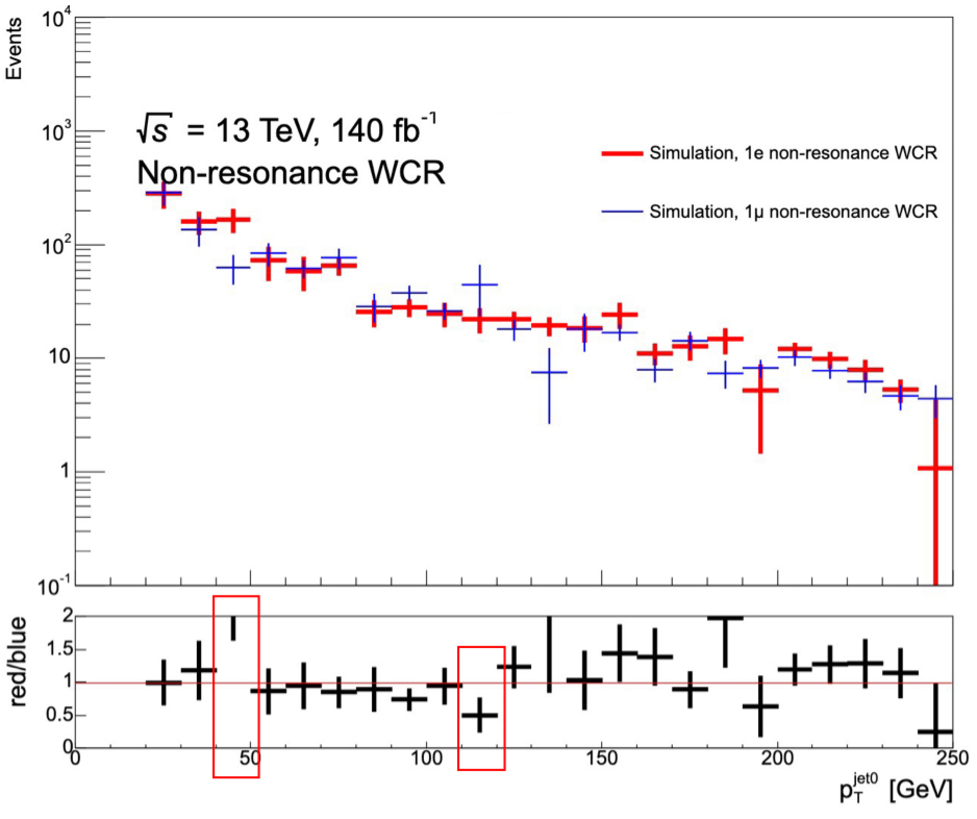
\includegraphics[width=\linewidth]{Figs/CH8/studies/WCR_emuRatio_MC.pdf}
        \caption[]{Simulation.}
    \end{subfigure}
    \caption[Electron and muon leading-jet momentum comparison]{Electron and muon channel comparison of leading jet $\pT$ in $\CRW$-$\NonRes$ for data (left) and MC (right). The red line shows the leading jet $\pT$ for the electron channel and the blue line shows the one for the muon channel. $2.6\sigma$ and $0.7\sigma$ discrepancies are observed for data and MC samples, respectively.}
    \label{fig:app_ch8_emu_ratio}
\end{figure}

\begin{figure}[htpb]
    \centering
    \begin{subfigure}{0.49\linewidth}
        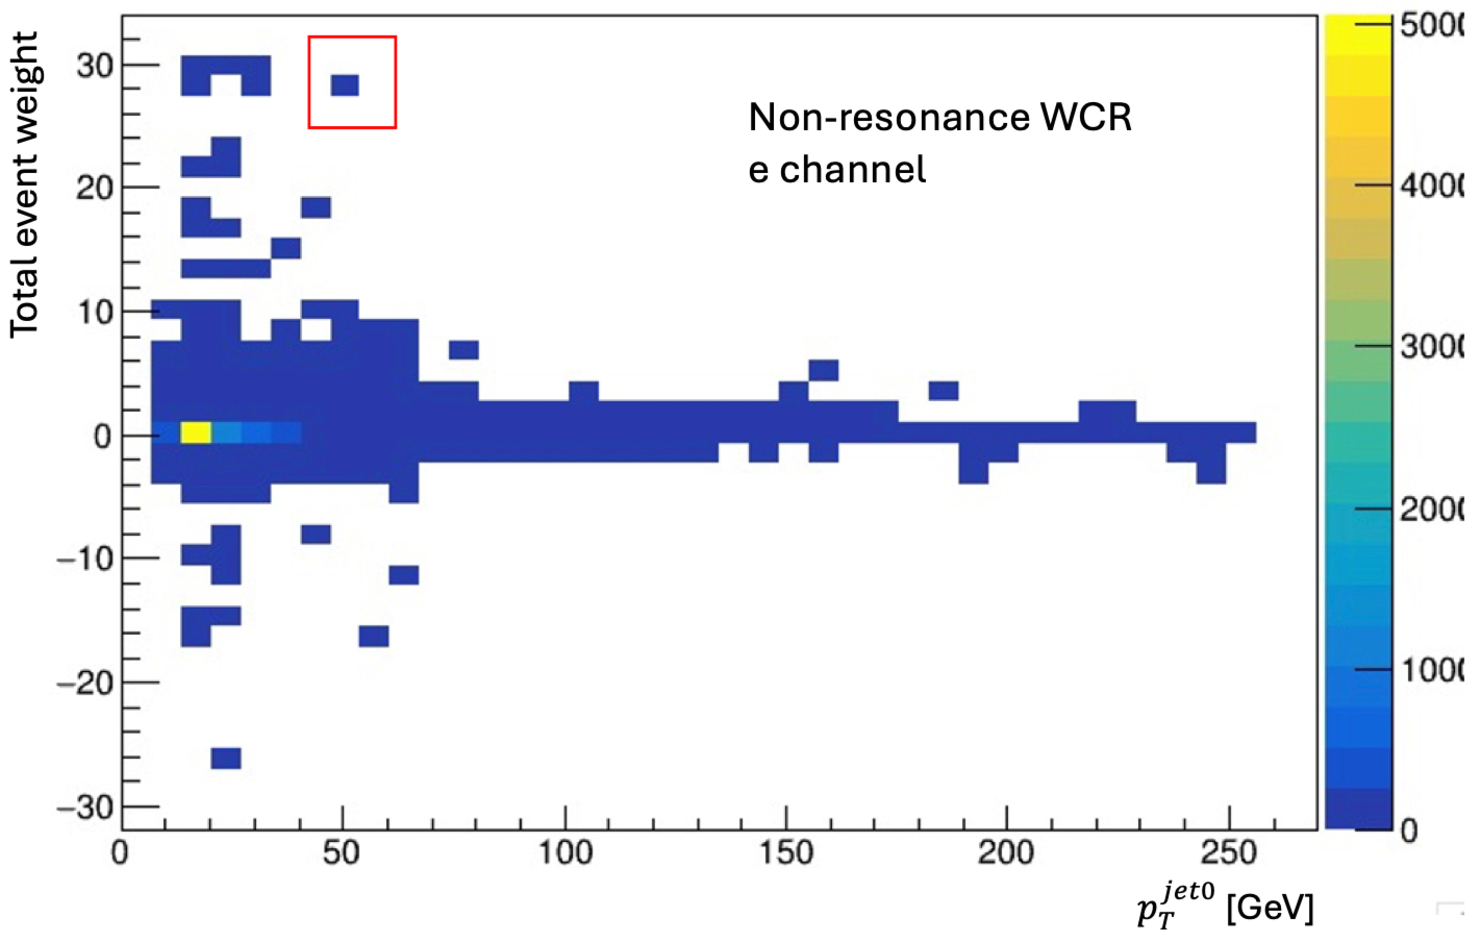
\includegraphics[width=\linewidth]{Figs/CH8/studies/WCR_evenweight_e.pdf}
        \caption[]{Electron channel.}
    \end{subfigure}\hfill
    \begin{subfigure}{0.49\linewidth}
        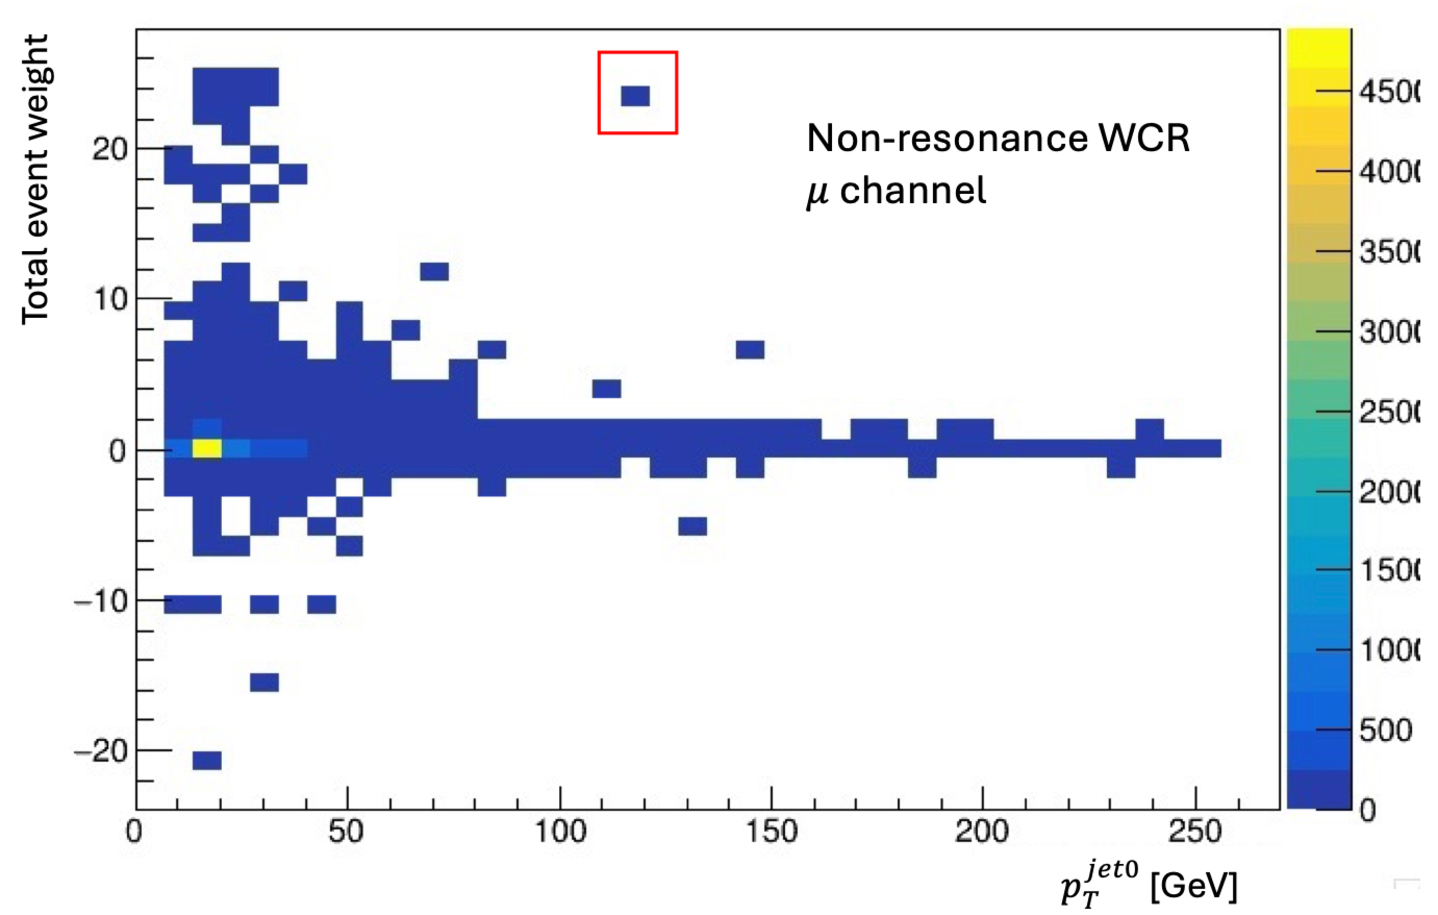
\includegraphics[width=\linewidth]{Figs/CH8/studies/WCR_evenweight_mu.pdf}
        \caption[]{Muon channel.}
    \end{subfigure}
    \caption[Simulated event weights in CRW-NonRes]{Event weight distribution as a function of leading jet $\pT$ in $\CRW$-$\NonRes$ for the electron (left) and muon (right) channels. Events that are marked with red rectangles correspond to the deviated bins marked in the simulation $e/\mu$ ratio distribution in Figure~\ref{fig:app_ch8_emu_ratio}.}
    \label{fig:app_ch8_emu_weights}
\end{figure}

